\documentclass{scrartcl}
\usepackage{tcolorbox}
\usepackage{tabularx}
\usepackage[sexy]{evan}
\usepackage{ltablex}
\newcommand\at[2]{\left.#1\right|_{#2}}
\declaretheorem[style=thmgreenbox,name=Notation,sibling = theorem]{notation}
\declaretheorem[style=thmgreenbox,name=Notation,numbered=no]{notation*}

\title{A guide to the \href{https://github.com/The-Academia-Kusanali-Mains/Kusanali-Bot}{Kusanali Bot's} commands}
\author{\text{bryanli\#2718}}
\date{June 2022}

\begin{document}

\maketitle
\tableofcontents
\newpage

\section{Moderation}
All mandatory options will be italicized, and optional ones will be in []
\subsection{Bans}[Requires mod and ban members perms]
\begin{tabularx}{\textwidth}{|>{\raggedright\arraybackslash}X|>{\raggedright\arraybackslash}X|}
\hline 
Command & Examples\\
\hline
/ban \textit{user(s)} [duration] [reason].

\begin{itemize}
    \item To ban a person, simply use the slash command ban.
    
    \item The members are simply the mentions or ids of the members you wish to ban. To mass ban, simply put multiple member references separated by a space in the member option. 

    \item The duration of their ban is simply a time string. To find more information, check out section \ref{time}.

    \item The reason is simply the reason for the ban. This will be logged and messaged to the offender(s). 
\end{itemize}
& \begin{enumerate}
    \item 
    /ban \color{black} user: \color{gray}436363390844403732 \color{black} 
    duration: \color{gray}10d \color{black}
    
    In this case, we are tempbanning the user 436363390844403732 for 10 days.
    \item
    /ban \color{black} user: \color{gray}$679102151653457941$ $906318377432281088$ $226092067737174026$ $185906419625623552$ \color{black}duration: \color{gray}December 21st, 2022 \color{black} reason: \color{gray} mod abooz pls demote\color{black}
    
    Now, we are mass banning 4 people until December 21st, 2022 for the reason "mod abooz pls demote."
\end{enumerate}\\
\hline
/unban \textit{user(s)} [reason]
\begin{itemize}
    \item Similar to /ban, use the slash command /unban to unban members. 
    
    \item Once again, you can also have multiple ids/mentions in the user option to mass unban
    
    \item The reason is an optional part that logs why you unbanned the individuals.
\end{itemize}&
\begin{enumerate}
    \item /unban \color{black} user: \color{gray} 436363390844403732 \color{black}
    Here, we are unbanning the user 436363390844403732.
    
    \item /unban \color{black} user: \color{gray} $679102151653457941$ $906318377432281088$ $226092067737174026$ $185906419625623552$ \color{black} reason: \color{gray} maybe you aren't so bad \color{black}
    
    Now, we are unbanning 4 people with the reason "maybe you aren't so bad."
\end{enumerate}
\\
\hline
/bans user(s)
\begin{itemize}
    \item To view a person's bans, simply use the command /bans.
    \item For this command, you may only provide one member.
\end{itemize}&
\begin{enumerate}
    \item /bans user: \color{gray}436363390844403732\color{black}
    
    This command lists all bans and unbans for the user $436363390844403732.$
\end{enumerate}\\
\hline
\end{tabularx}

\subsection{Warns} [Requires trial mod and manage message perms]
\begin{tabularx}{\textwidth}{|>{\raggedright\arraybackslash}X|>{\raggedright\arraybackslash}X|}
\hline 
Command & Examples\\
\hline
/warn \textit{user(s)} \textit{reason.}

\begin{itemize}
    \item To warn a person, simply use the slash command warn.
    
    \item The warn command functions very similarly to kicks, and will dm the warn reason to the members. Note that the reason is mandatory this time. 
\end{itemize}
& \begin{enumerate}
    \item 
    /warn \color{black} user: \color{gray}436363390844403732 \color{black} reason: \color{gray}stinky go wear deodorant\color{black}
    
    In this way, we are warning the user 436363390844403732 for "stinky go wear deodorant."
    \item
    /warn \color{black} user: \color{gray}$679102151653457941$ $906318377432281088$ $226092067737174026$ $185906419625623552$ \color{black} reason: \color{gray} talking about fetishes \color{black}
    
    Now, we are warning 4 users for "talking about fetishes."
\end{enumerate}\\
\hline
/pardon \textit{user(s)} [reason]
\begin{itemize}
    \item Unlike unban, we use the command pardon to remove warns. 
    
    \item This will show each warn for every user and allow you to select the desired warn to pardon.
\end{itemize}&
\begin{enumerate}
    \item /pardon user: \color{gray} 752939152273834086  \color{black}
    
    Now, a selection screen with all the user's warns will appear 
\end{enumerate}
\begin{center}
    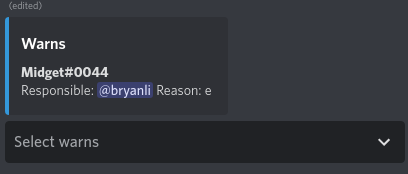
\includegraphics[width=2in]{images/pardon.png}
\end{center}
\indent Now, simply select the warn you wish to pardon.
\\
\hline
/warns user(s)
\begin{itemize}
    \item To view a person's warns, simply use the command /warns.
    \item For this command, you may only provide one member.
\end{itemize}&
\begin{enumerate}
    \item /warns user: \color{gray}436363390844403732\color{black}
    
    This command lists all warns and pardoned for the user $436363390844403732.$
\end{enumerate}\\
\hline
\end{tabularx}
\newpage
\subsection{Notes} [Requires trial mod and manage message perms]
\begin{tabularx}{\textwidth}{|>{\raggedright\arraybackslash}X|>{\raggedright\arraybackslash}X|}
\hline 
Command & Examples\\
\hline
/note \textit{user(s)} \textit{reason.}

\begin{itemize}
    \item All in all, notes and warns function identically. It is just that notes will not be dm'd to the member.
\end{itemize}
& \begin{enumerate}
    \item 
    /note \color{black} user: \color{gray}436363390844403732 \color{black} reason: \color{gray}stinky go wear deodorant\color{black}
    
    In this way, we are writing a note for the user 436363390844403732 saying "stinky go wear deodorant."
    \item
    /note \color{black} user: \color{gray}$679102151653457941$ $906318377432281088$ $226092067737174026$ $185906419625623552$ \color{black} reason: \color{gray} talking about fetishes \color{black}
    
    Now, we are warning 4 users for "talking about fetishes."
\end{enumerate}\\
\hline
/omit \textit{user(s)} [reason]
\begin{itemize}
    \item Like pardon, the command to remove notes is omit.
\end{itemize}&
\begin{enumerate}
    \item /omit user: \color{gray} 752939152273834086  \color{black}
    
    Now, a selection screen with all the user's notes will appear 
\end{enumerate}
\begin{center}
    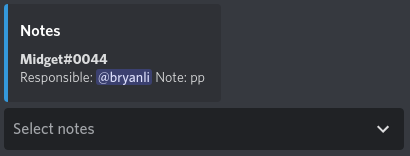
\includegraphics[width=2in]{images/omit.png}
\end{center}
\indent Now, simply select the note you want to delete.
\\
\hline
/notes \textit{user(s)}
\begin{itemize}
    \item To view a person's notes, simply use the command /notes.
    \item For this command, you may only provide one member.
\end{itemize}&
\begin{enumerate}
    \item /notes user: \color{gray}436363390844403732\color{black}
    
    This command lists all current notes for the user $436363390844403732.$
\end{enumerate}\\
\hline
\end{tabularx}
\newpage

\subsection{Mutes} [Requires trial mod and manage message perms]
\begin{tabularx}{\textwidth}{|>{\raggedright\arraybackslash}X|>{\raggedright\arraybackslash}X|}
\hline 
Command & Examples\\
\hline
/mute \textit{user(s)} [duration] [reason].

\begin{itemize}
    \item Muting works very similarly to bans. All the users roles will be removed and replaced by the mute role which can be set via /setmute.
    
    \item The members are simply the mentions or ids of the members you wish to mute. To mass mute, simply put multiple member references separated by a space in the member option. 

    \item The duration of their mute is simply a time string. To find more information, check out section \ref{time}. If no duration is specified, the mute will be permanent

    \item The reason is simply the reason for the mute. This will be logged and messaged to the offender(s). 
\end{itemize}
& \begin{enumerate}
    \item 
    /mute \color{black} user: \color{gray}436363390844403732 \color{black} 
    duration: \color{gray}10d \color{black}
    
    In this case, we are tempbanning the user 436363390844403732 for 10 days.
    \item
    /ban \color{black} user: \color{gray}$679102151653457941$ $906318377432281088$ $226092067737174026$ $185906419625623552$ \color{black}duration: \color{gray}December 21st, 2022 \color{black} reason: \color{gray} shut up bozo\color{black}
    
    Now, we are muting 4 people until December 21st, 2022 for the reason "shut up bozo."
\end{enumerate}\\
\hline
/unmute \textit{user(s)} [reason]
\begin{itemize}
    \item If you wish to unmute a user, simply use the slash command /unmute.

    \item You may unmute multiple users at a time by supplying multiple members separated by a space in the users category. 
\end{itemize}&
\begin{enumerate}
    \item /unmute \color{black} user: \color{gray} 436363390844403732 \color{black}
    Here, we are unmuting the user 436363390844403732.
    
    \item /unmute \color{black} user: \color{gray} $679102151653457941$ $906318377432281088$ $226092067737174026$ $185906419625623552$ \color{black} reason: \color{gray} wait i need yall to work \color{black}
    
    Now, we are unmuting 4 people with the reason "wait i need yall to work."
\end{enumerate}
\\
\hline
/mutes user(s)
\begin{itemize}
    \item To view a person's mute history, simply use the command /mutes.
    \item For this command, you may only provide one member.
\end{itemize}&
\begin{enumerate}
    \item /mutes user: \color{gray}436363390844403732\color{black}
    
    This command lists all mutes and unmutes for the user $436363390844403732.$
\end{enumerate}\\
\hline
\end{tabularx}


\subsection{Kicks} [Requires trial mod and kick member perms]
\begin{tabularx}{\textwidth}{|>{\raggedright\arraybackslash}X|>{\raggedright\arraybackslash}X|}
\hline 
Command & Examples\\
\hline
/kick \textit{user(s)}
\begin{itemize}
    \item Similar to how bans work, to kick a member you can specify one or a list of members to kick as well as the reason for the kick
    \item The reason will be messaged and logged.
\end{itemize}
&
\begin{enumerate}
    \item /kick user: \color{gray}436363390844403732\color{black} 
    
    The only usage difference with bans is that no duration can be specified.
    \item /kick \color{black} user: \color{gray}$679102151653457941$ $906318377432281088$ \color{black} reason: \color{gray} byyyye\color{black}
    
    Similarly, we can also mass kick; however, this command will not be often used.
    
\end{enumerate}\\
\hline
/kicks \textit{user}
\begin{itemize}
    \item You check the kick history of a user by running the command /kicks. This can only accept one member (not a whole list).
\end{itemize}
&
\begin{enumerate}
    \item /kicks user: \color{gray}436363390844403732\color{black} 
    
    This will list all the kicks of 436363390844403732
\end{enumerate}\\
\hline

\end{tabularx}
\newpage
\subsection{Purge/Mass Delete} [Requires trial mod and manage message perms]
\begin{tabularx}{\textwidth}{|>{\raggedright\arraybackslash}X|>{\raggedright\arraybackslash}X|}
\hline
Command & Examples\\
\hline
/purge \textit{number} [user]

\begin{itemize}
    \item This command will delete the \textit{number} most recent messages in a channel
    
    \item If a user is supplied, only messages from the user in the \textit{number} most recent messages will be deleted
    
    \item This command will always ignore pinned messages.
\end{itemize}
&
\begin{enumerate}
    \item /purge number: \color{gray} 100\color{black}
    
    This command will purge the 100 most recent messages in the current channel ignoring pinned messages.
    
    \item /purge number: \color{gray} 999 \color{black} user: \color{gray} 436363390844403732 \color{black}
    
    In the 999 most recent messages in the channel, all messages by the user 436363390844403732 that aren't pinned will be deleted. 
\end{enumerate}\\
\hline

\end{tabularx}

\subsection{Slowmode} [Requires mod and manage channels perms]
\begin{tabularx}{\textwidth}{|>{\raggedright\arraybackslash}X|>{\raggedright\arraybackslash}X|}
\hline
Command & Examples\\
\hline
/slowmode \textit{duration} [channel]

\begin{itemize}
    \item To set the slowmode in a channel, run the command /slowmode.
    
    \item If no channel is supplied, the channel will be the one the command is run in.
    
    \item The duration is an combination of time in the format []h[]m[]s. 
    
    \item The maximum duration is 6 hours.
\end{itemize}
&
\begin{enumerate}
    \item /slowmode duration: \color{gray} 5s \color{black}
    
    This command sets the slowmode to 5 seconds. 
    
    \item /slowmode duration: \color{gray} 3h \color{black} channel: \color{gray} #general-chat \color{black}
    
    This command will set the slowmode in the channel #general-chat to 3 hours. 
\end{enumerate}\\
\hline

\end{tabularx}
\newpage
\section{Modmail} [Requires Mod and manage thread perms]
Once a new modmail is created, you will be added to a private thread. In this thread, you can safely send any message to discuss the contents of the modmail. 

\begin{tabularx}{\textwidth}{|>{\raggedright\arraybackslash}X|>{\raggedright\arraybackslash}X|}
\hline
Commands&Examples\\
\hline
/reply \textit{message}
\begin{itemize}
    \item To respond to a message, use the slash command reply.
    \item In general, please try to make it so one person continually replies. The only exceptions to this rule are when the original replier goes AFK or an admin is needed.
    \item Also, send your message in the channel before hand and get approval from your fellow mods/admins before sending.
    
\end{itemize}
& \begin{enumerate}
    \item /reply message: \color{gray} Hey! How can we help you! \color{black}
    
    Here, we are simply sending the message "Hey! How can we hlep you!" in the user's dm. 
\end{enumerate}\\
\hline
/delete
\begin{itemize}
    \item Doing this will delete the most recent message in the modmail.
    \item You may continually call /delete until there are no more messages to delete. 
    \item You will still be able to view the message, but the user will not
\end{itemize}
&
\begin{center}
    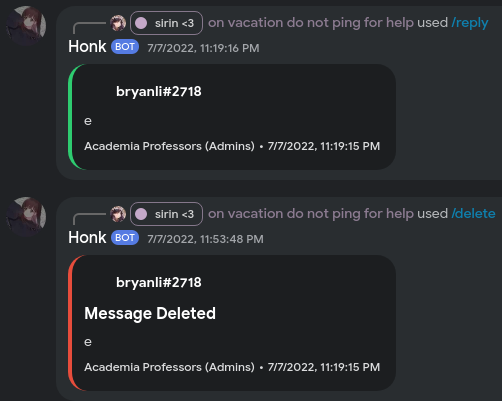
\includegraphics[width=2in]{images/modmail/delete.png}
\end{center}
Notice that you (the mod) can still see the original message\\
\hline
/end
\begin{itemize}
    \item To end a modmail, simply run the command /end. 
    \item You can also manually archive a thread to close it.
    \item When you end a modmail, it will dm the user Session ended!
\end{itemize}
&
\begin{enumerate}
    \item When you run the command /end, the message "Session ended!" will be sent in the channel. The thread will be archived after 5 seconds.
\end{enumerate}\\
\hline
\end{tabularx}
\newpage
\section{Ranks} 
The bot also can track leveling. One exp is added every time a "conversation" occurs. A conversation is simply when one person sends a message after a different person. This way, people simply spamming bots or talking to themselves will not gain exp. The level system is quadratic and follows the equation $20x^2+300x+200.$ If you wish, you may alter the coefficients \href{https://github.com/Bryli06/KusanaliBot/blob/main/core/calculate_level.py}{here.}

All level related commands will start with /level

\begin{tabularx}{\textwidth}{|>{\raggedright\arraybackslash}X|>{\raggedright\arraybackslash}X|}
\hline 
Command & Examples\\
\hline
/level events [Requires trial mod]
\begin{itemize}
    \item This will list all level events in the server. Level events are adding or removing a role when a member hits a certain level.
\end{itemize}
&
\begin{enumerate}
    
\end{enumerate}\\
\hline
/level set \textit{user} \textit{mode} \textit{amount} [Requires administrator]
\begin{itemize}
    \item You can set the exp or level of a member using the command /level set.
    \item The mode is either exp or level so you can either set a members level amount or exp amount.
    \item The amount is simply whatever value to set it to
\end{itemize}
&
\begin{enumerate}
    \item /level set user: \color{gray} 436363390844403732 \color{black} mode: \color{gray}Level \color{black} amount: \color{gray} 200 \color{black}
    
    Here, we are setting the level of 436363390844403732 to 200. Remember, this sets the level not adds the level. 
\end{enumerate}\\
\hline

\end{tabularx}
\newpage
\section{Automod}
All commands in this section will start with /banlist \textit{command}

\begin{tabularx}{\textwidth}{|>{\raggedright\arraybackslash}X|>{\raggedright\arraybackslash}X|}
\hline
Command & Examples\\
\hline
/banlist show [Requires mod]
\begin{itemize}
    \item Shows all the banned words and their corresponding flags
\end{itemize}
&
\begin{enumerate}
    \item /banlist show 
\end{enumerate}\\
\hline
/banlist add \textit{word} [Requires admin]
\begin{itemize}
    \item This adds the word to the ban list.
    \item A secondary screen will appear that allows you to select the flags.
    \item There are currently 3 flags implemented: case, delete, and whole.
    \item Case means that the word must be case specific. Therefore, if the word "luma" was banned with the flag case, Luma wouldn't be triggered as the letter "L" is capitalized.
    \item Delete simply specifies that the word will be deleted if detected.
    \item Whole requires the word to appear on its own. So, if the word "luma" was banned with the flag whole, "aesnuhaoeu\textbf{luma}sthou" would not trigger the automod as it is not on its own. On the other hand, "aesnuhaoeu luma sthou" would.
\end{itemize}
&
\begin{enumerate}
    \item /banlist add banned\_word: \color{gray} luma \color{black}
    
\end{enumerate}
    Running this command brings up a new menu to select flags
\begin{center}
        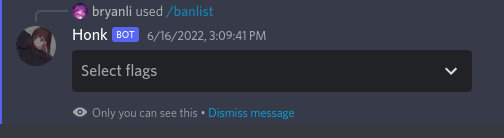
\includegraphics[width=2in]{images/banlist/select.png}
\end{center}
Now, click on the select flags menu
\begin{center}
    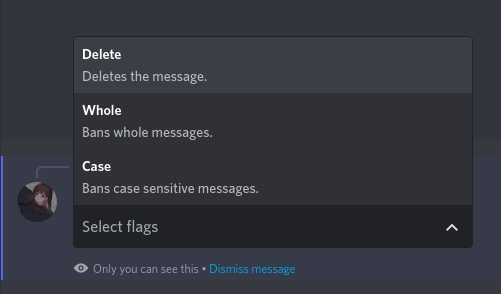
\includegraphics[width=2in]{images/banlist/flags.png}
\end{center}
Choose whichever flags you wish to add to the banned word.
\begin{center}
    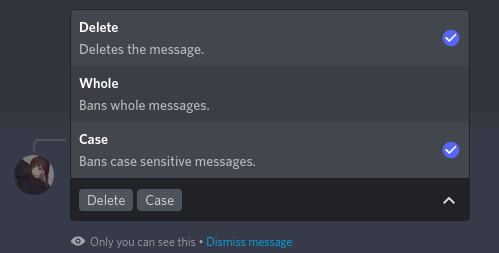
\includegraphics[width=2in]{images/banlist/selected.png}
\end{center}
To submit the flags, simply click outside the menu to take the focus away.
\begin{center}
    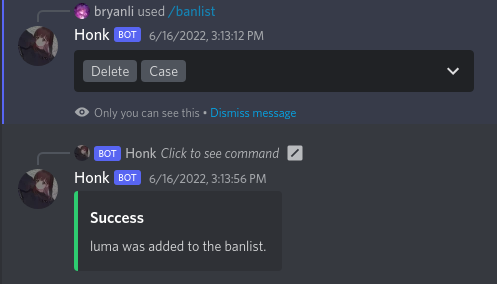
\includegraphics[width=2in]{images/banlist/added.png}
\end{center}
\\
\hline
/banlist remove \textit{word} [Requires Admin]
\begin{itemize}
    \item This command will remove a word from the banlist. 
    \item If the word is not a banned word, the application will not respond
\end{itemize}&
\begin{enumerate}
    \item /banlist remove banned\_word: \color{gray} luma \color{black}
    
    Running this command removes the word luma from the banned words
    
    \item /banlist remove banned\_word: \color{gray} banana \color{black}
    
    In the case that the word is not banned, like the term banana, the bot will have the error 
\end{enumerate}
\begin{center}
    
\includegraphics[width=2in]{images/banlist/no respond.png}
\end{center}
\hline
\end{tabularx}

\newpage
\section{Giveaways} [Requires event admin]
\begin{tabularx}{\textwidth}{|>{\raggedright\arraybackslash}X|>{\raggedright\arraybackslash}X|}
\hline
Format & Examples \\
\hline
/giveaway create \textit{reward winners end} [required\_roles] [banned\_roles] [tickets]
\begin{itemize}
    \item This creates a giveaway with the prize of \textit{reward}. 
    \item \textit{winners} number of winners will be chosen at the end.
    \item The giveaway will end at {end} which is a human readable string.
    \item There are 3 optional requirements: required roles, banned roles, and tickets.
    \item required\_roles is a list of roles that each entrance must have. Members will only need to have one of the roles listed.
    \item banned\_roles is a list of roles that are prohibited from participating. If a member has any of the banned roles, they will not be considered. 
    \item tickets allow you to give extra tickets to certain roles. Simply specify a role followed by the ticket amount. 
\end{itemize}
&
\vspace{0.25cm}
/giveaway create reward: \color{gray}welkin \color{black} winners: \color{gray}1 \color{black}end: \color{gray} 1d \color{black} required\_roles: \color{gray}@Academy Aspires \color{black} banned\_roles: \color{gray} @mute \color{black} tickets: \color{gray} @Team Kusanali 30 @Team YaoYao 10 @Team Kuki 10 \color{black}

\vspace{0.5cm}
In this case, we are creating a giveaway for 1 welkin that requires members to have the role Academy Aspires. Any member with the role mute will not be allowed to join and members with the role Team Kusanali will gain 30 extra tickets. Similarly, both Team YaoYao and Kuki will recieve 10 extra tickets.
    
Now, we will be previewed the giveaway and can confirm or deny it before sending it out. 
\begin{center}
    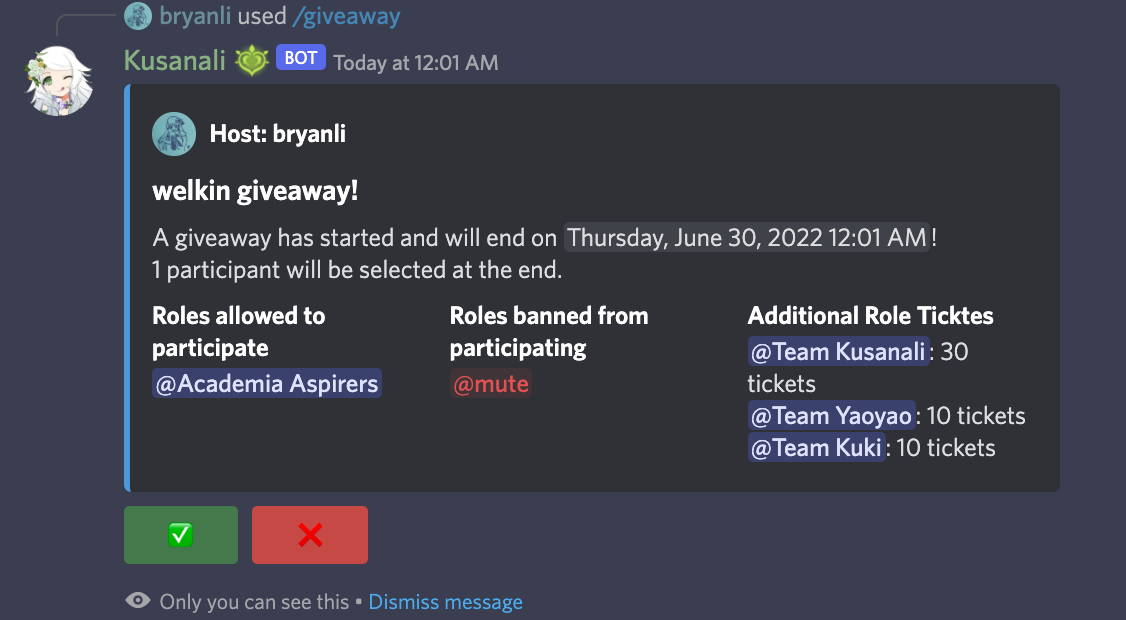
\includegraphics[width=2in]{images/giveaway.png}
\end{center}
Note that you only have $60$ seconds to confirm the giveaway before it becomes inactive!
\\
\hline 
/giveaway end \textit{message\_id}
\begin{itemize}
    \item Sometimes, you wish to prematurely end a giveaway. To do this you can use the giveaway end command.
    \item The message id is the id of the giveaway message. See \href{https://support.discord.com/hc/en-us/articles/206346498-Where-can-I-find-my-User-Server-Message-ID-}{here} for more info. 
\end{itemize}&
\vspace{0.25cm}
Assume that there is a giveaway going on with message id $991539009664852039$ that we wish to end early. To do this, all we need to do is run the command:
\newline
\vspace{0.25cm}
/giveaway end message\_id: \color{gray} 991539009664852039 \color{black}
\\
\hline
\end{tabularx}
Important: Giveaway is a constantly updated cog. New commands like reroll may be introduced before this guide is updated. Please use your common sense! 
\newpage
\section{Time management} \label{time}
There are 2 ways to denote time: (1) using the duration format, or (2) a human readable string.

\begin{tabularx}{\textwidth}{|>{\raggedright\arraybackslash}X|>{\raggedright\arraybackslash}X|}
\hline
Format & Examples \\
\hline
Duration Format

\begin{itemize}
    \item The duration format is simply any duration in the form []y[]mo[]w[]d[]m[]s.
    
    \item Here [] is an integer, y - years, mo - months, w - weeks, d - days, m - minutes, and s - seconds.
    
    \item Flags may be dropped if they are not needed, but they can not be written in a different order. 
    
\end{itemize}&
\begin{enumerate}
    \item 3d2m1s
    
    Here we are specifying a duration of 3 days 3 minutes and 1 seconds.
    
    \item 3d2mo1m
    
    Here, we are trying to denote a time of 3 days 2 months and 1 minutes; however. this will only parse as 3 days since the keys are not in the correct order. 
    
    \item 120m61s
    
    Now, we are trying to use a duration of 120 minutes and 61 seconds. Notice that this is the same as 2h1m1s, however, this will parse the same.
    
    
\end{enumerate}\\
\hline
Human Readable String 
\begin{itemize}
    \item There are many different types of Human readable strings, but in general, most date strings will work.
    \item This includes dates, relative dates, and even other languages
    \item Dates are simply and string that represent a date. It can include the time, the date, and the timezone. 
    \item On the other hand, relative dates are simply strings that tell time relative to the current time. Think "in 3 days" or "tomorrow."
    \item As mentioned before, the parser can accept strings in other languages such as chinese if you are interested. 
\end{itemize}& 
\begin{enumerate}
    \item 12/12/12
    
    Here we are simply specifying the date December 12, 2012 using a date string. The date parser defaults to M-D-Y, so be careful if you are used to D-M-Y. We can also explain it verbosely,
    
    \item Friday, 12 Dec 2014 10:55:50
    
     Now, we have used a full string to specify the date December 12th, 2014 at 10:55:50 AM.
    \item in two hours
    
    Here we are using a relative date. This will parse into whatever the time will be in 2 hours.
    
\end{enumerate}\\
\hline
\end{tabularx}
\newpage
\section{Miscellaneous}
\begin{tabularx}{\textwidth}{|>{\raggedright\arraybackslash}X|>{\raggedright\arraybackslash}X|}
\hline
Format & Examples \\
\hline
/countdown create \textit{name} \textit{end} [Requires owner]
\begin{itemize}
    \item The name is simply whatever the countdown you wish to be called. The final vc's name will be {name}: {time until end}
    \item The end is simply a time duration. 
\end{itemize}&
\begin{enumerate}
    \item /countdown create name: \color{gray} Time until Kusanali drop \color{black} end: \color{gray} October 5th, 2022 \color{black}
    
    This will create a vc called "Time until Kusanali drop: 3 months." The duration "3 months" will update as time passes. You may freely move the channel around as long as Kusanali has permission to view. 
    
\end{enumerate}\\
\hline
\end{tabularx}
\end{document}

\end{document}
